% report.tex
% Report on summer 2009 four weeks practice.
% Vladimir Rutsky <altsysrq@gmail.com>
% 08.09.2009

\documentclass[a4paper,12pt,titlepage]{report}

% Encoding support.
\usepackage{ucs}
\usepackage[utf8x]{inputenc}
\usepackage[T2A]{fontenc}
\usepackage[russian]{babel}

\usepackage{amsmath, amsthm, amssymb}

\usepackage{graphicx} 

% Indenting first paragraph.
\usepackage{indentfirst}

% Spaces after commas.
\frenchspacing
% Minimal carrying number of characters,
\righthyphenmin=2

% From K.V.Voroncov Latex in samples, 2005.
\textheight=24cm   % text height
\textwidth=16cm    % text width.
\oddsidemargin=0pt % left side indention
\topmargin=-1.5cm  % top side indention.
\parindent=24pt    % paragraph indent
\parskip=0pt       % distance between paragraphs.
\tolerance=2000
%\flushbottom       % page height aligning
%\hoffset=0cm
%\pagestyle{empty}  % without numeration

\begin{document}

% Title page.
\begin{titlepage}
\newpage

\begin{center}
% TODO: What is `\\*'?
% TODO: Year.
% TODO: Add place for scientific advicer signature.
% TODO: Increase font.
% TODO: Vertically align center text.
САНКТ-ПЕТЕРБУРГСКИЙ \\*
ГОСУДАРСТВЕННЫЙ ПОЛИТЕХНИЧЕСКИЙ УНИВЕРСИТЕТ \\*
\hrulefill
\end{center}

\flushright{КАФЕДРА ПРИКЛАДНОЙ МАТЕМАТИКИ}

\vspace{1cm}
\vspace{8em}

\begin{center}
\Large{Отчет \\ о летней практике}
\end{center}

\vspace{2.5em}

\begin{center}
Студента группы 4057/2 \\ Руцкого Владимира
\end{center}

\vspace{14em}

\begin{flushleft}
Куратор, \\
магистр кафедры ...  \hfill Ковалёв~А.\,С.
\end{flushleft}

\vspace{\fill}

\begin{center}
Санкт-Петербург \\ 2009
\end{center}

\end{titlepage}
\pagebreak

% Content

\section*{Постановка задачи}
Дано: множество контуров $C$, контур $K$.

Пусть $T(X)$~--- триангуляция множества контуров $X$.

Пусть $S(A, X) = \{ x | x = A \setminus c, c \in X \}$. Обозначим $C' = S(K, C)$

Пусть $P(T, \varepsilon) = \{ t_i | s(t_i) <  \varepsilon, t_i \in T \}$, где $t_i$~--- треугольник триангуляции $T$, 
$s(t_i)$~--- его площадь.

$|P(T(C'), \varepsilon)|$ оказывается неоправданно велико.

\begin{figure}[htp]
\centering
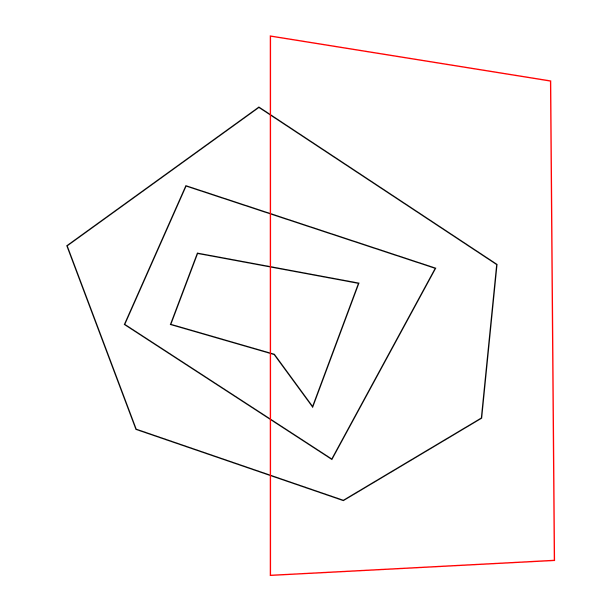
\includegraphics[width=8cm, height=8cm]{orig_contours.pdf}
\caption{$C$~--- черные, $K$~--- красный}\label{fig:orig_contours}
\end{figure}

\begin{figure}[htp]
\centering
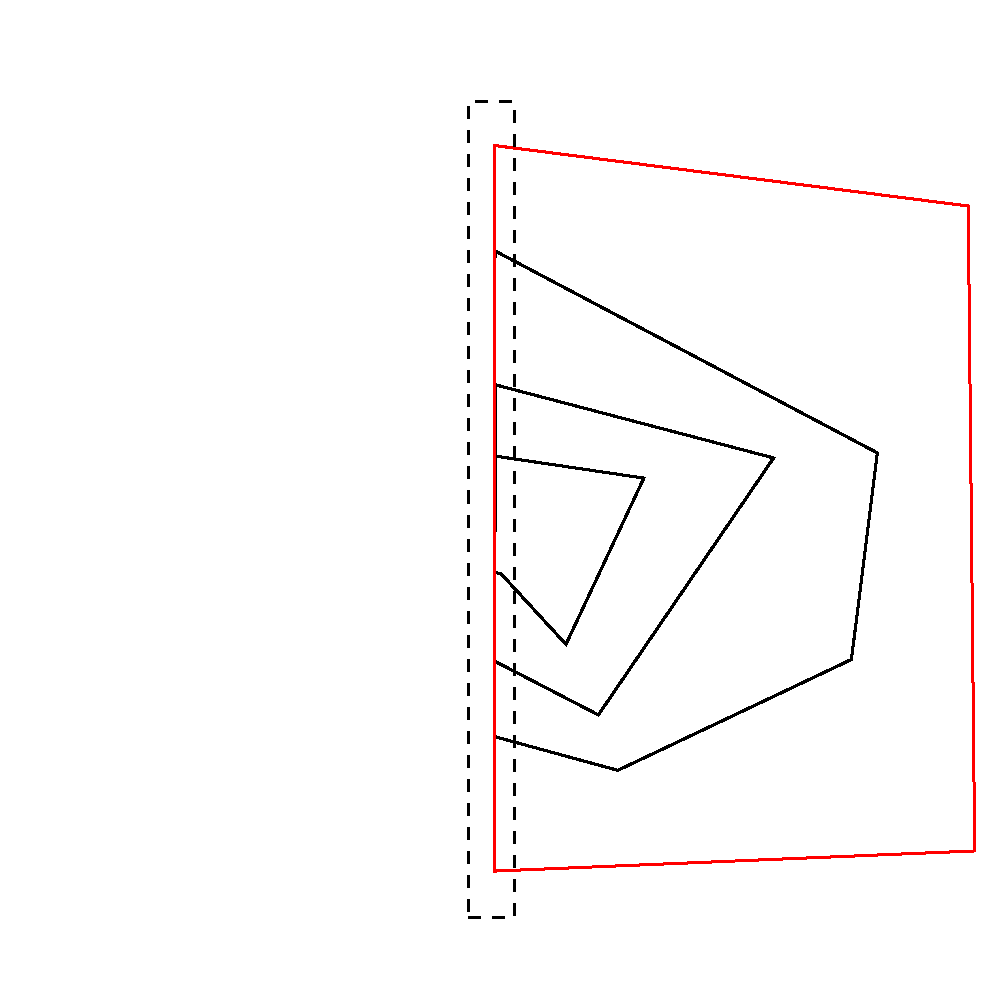
\includegraphics[width=8cm, height=8cm]{cutted_contours.pdf}
\caption{$C' = $ (черные)~--- результат сечения контуров $C$ контурами $K$}\label{fig:cutted_contours}
\end{figure}

Дано: множество контуров $C$, множество секущих контуров $K$.
Контура из $C$ секутся контурами из $K$, полученное множество контуров $C'$ 
подаётся на вход алгоритм триангуляции.

В результате сечения часто возникают ситуации, когда несколько контуров из $C'$ будут граничить по ребру, 
но при этом не иметь общих вершин. Обозначим множество таких смежных по ребру контуров $A$.

Из-за неточности представления вещественных чисел в компьютере,
смежность будет нестрогой, как показано на Рис. \ref{fig:zoomed_contours}.
\begin{figure}[htp]
\centering
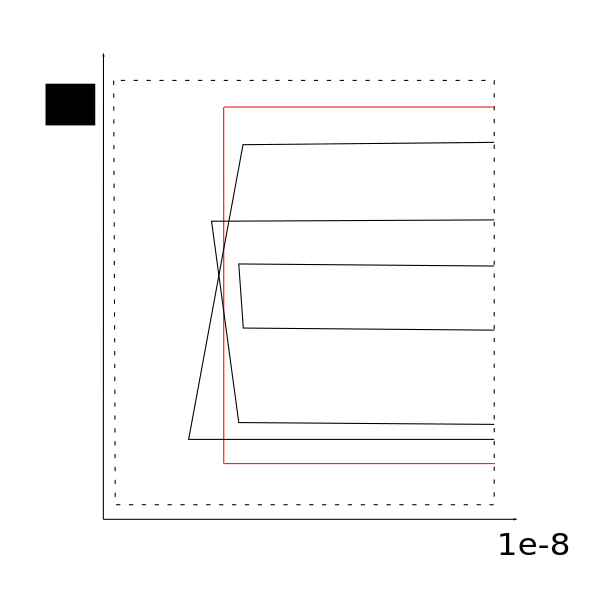
\includegraphics[width=8cm, height=8cm]{zoomed_contours.pdf}
\caption{Нестрогая смежность контуров из $A$ (увеличенная по оси $X$, обозначенная пунктиром область сечения с Рис. \ref{fig:cutted_contours})}\label{fig:zoomed_contours}
\end{figure}
В триангуляции такие контура дадут длинные вытянутые треугольники $T_\varepsilon$, с практически нулевой площадью, 
как показано на Рис. \ref{fig:triangulation}.
\begin{figure}[htp]
\centering
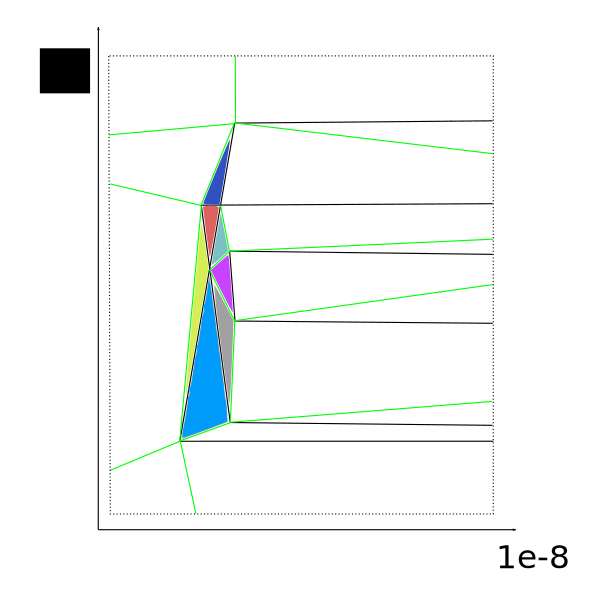
\includegraphics[width=8cm, height=8cm]{triangulation.pdf}
\caption{Вытянутые треугольники $T_\varepsilon$ залиты (увеличенная по оси $X$, обозначенная пунктиром область сечения с Рис. \ref{fig:cutted_contours})}\label{fig:triangulation}
\end{figure}

Задача: модифицировать входные данные таким образом,
чтобы в конечной триангуляции не было треугольников $T_\varepsilon$, 
возникающих из-за сечения, как показано выше.

%\includegraphics[width=10cm]{t-vertices}
%\epsfbox{t-vertices.eps}
%\includegraphics[width=12cm, height=16cm]{t-vertices.pdf}
%\includegraphics[width=12cm]{t-vertices.pdf}
%\input{t-vertices}

%\begin{center}
%\includegraphics[width=12cm, height=12cm]{t-vertices.pdf}
%\end{center}

\section*{Выбранный метод решения}
Было решено подразбить рёбра контуров $A$ так, 
чтобы все контура из $A$ касались друг друга строго по общим рёбрам.

Для этого рассмотрим каждое ребро $e$ каждого контура $c$ из $A$.
Оно перекрывается с множеством рёбер $A_e$ контуров $A$.
Рассмотрим все вершины $v$ рёбер $A_e$, если $v$ лежит близко к $e$, 
подразобьём $e$ вершиной $v$.

Если два контура $a_1$, $a_2$ касались по перекрывающимся рёбрам $e_1$, $e_2$, 
то после работы алгоритма они будут перекрываться по новой общей части подразбиения $e_1$, $e_2$.

Оптимизация поиска смежных по рёбрам контуров $A_e$ была выполнена с использованием 
двухуровневых сеток.

\section*{Результаты}
Были получены результаты следующего порядка: 
на сцене c количеством контуров $|C|=70 \cdot 10^3$,
количеством секущих контуров $|K|=6 \cdot 10^3$ 
было внесено $5 \cdot 10^3$ дополнительных вершин в контура $C'$. 

После обработки входных данных построенным алгоритмом, 
в конечной триангуляции не оказалось длинных, 
вытянутых треугольников на границе секущих контуров $K$.

% Quick and dirty.
% TODO
\begin{thebibliography}{9}
\bibitem{prepara-sheimos}
  Ф.~Препарата, М.~Шеймос
  \emph{Вычислительная геометрия: Введение}.
  Мир,
  1989.
\bibitem{kormen}
  Т.\,Х.~Кормен, Ч.\,И.~Лейзерсон
  \emph{Алгоритмы: построение и анализ.}
  Вильямс,
  2-е издание,
  2008.
\end{thebibliography}

\end{document}
